% Created 2023-04-19 сре 00:41
% Intended LaTeX compiler: pdflatex
\documentclass[11pt]{article}
\usepackage[utf8]{inputenc}
\usepackage[T1]{fontenc}
\usepackage{graphicx}
\usepackage{longtable}
\usepackage{wrapfig}
\usepackage{rotating}
\usepackage[normalem]{ulem}
\usepackage{amsmath}
\usepackage{amssymb}
\usepackage{capt-of}
\usepackage{hyperref}
\author{John Doe}
\date{\today}
\title{Programming exercises}
\hypersetup{
 pdfauthor={John Doe},
 pdftitle={Programming exercises},
 pdfkeywords={},
 pdfsubject={},
 pdfcreator={Emacs 28.2 (Org mode 9.6.1)}, 
 pdflang={English}}
\usepackage{biblatex}

\begin{document}

\maketitle
\tableofcontents


\section{Browser history}
\label{sec:org649a689}
You have a browser of one tab where you start on the homepage and you can visit another url, get back in the history
number of steps or move forward in the history number of steps.

\subsection{Implement the \texttt{BrowserHistory} class:}
\label{sec:org96a65b9}

\begin{description}
\item[{\texttt{BrowserHistory(string homepage)}}] Initializes the object with the homepage of the browser.
\item[{\texttt{void visit(string url)}}] Visits \texttt{url} from the current page. It clears up all the forward history.
\item[{\texttt{string back(int steps)}}] Move \texttt{steps} back in history. If you can only return \texttt{x} steps in the history and \texttt{steps > x}, you will return only \texttt{x} steps.
Return the current \texttt{url} after moving back in history at most \texttt{steps}.
\item[{\texttt{string forward(int steps)}}] Move \texttt{steps} forward in history. If you can only forward \texttt{x steps} in the history and \texttt{steps > x}, you will forward only \texttt{x steps}.
Return the current \texttt{url} after forwarding in history at most \texttt{steps}.
\end{description}

\subsection{Example}
\label{sec:org9c7c2bc}
\begin{verbatim}
Input:
["BrowserHistory","visit","visit","visit","back","back","forward","visit","forward","back","back"]
[["mig.mk"],["google.com"],["facebook.com"],["youtube.com"],[1],[1],[1],["linkedin.com"],[2],[2],[7]]

Output:
[null,null,null,null,"facebook.com","google.com","facebook.com",null,"linkedin.com","google.com","mig.mk"]

Explanation:
BrowserHistory browserHistory = new BrowserHistory("mig.mk");
browserHistory.visit("google.com");       // You are in "mig.mk". Visit "google.com"
browserHistory.visit("facebook.com");     // You are in "google.com". Visit "facebook.com"
browserHistory.visit("youtube.com");      // You are in "facebook.com". Visit "youtube.com"
browserHistory.back(1);                   // You are in "youtube.com", move back to "facebook.com" return "facebook.com"
browserHistory.back(1);                   // You are in "facebook.com", move back to "google.com" return "google.com"
browserHistory.forward(1);                // You are in "google.com", move forward to "facebook.com" return "facebook.com"
browserHistory.visit("linkedin.com");     // You are in "facebook.com". Visit "linkedin.com"
browserHistory.forward(2);                // You are in "linkedin.com", you cannot move forward any steps.
browserHistory.back(2);                   // You are in "linkedin.com", move back two steps to "facebook.com" then to "google.com". return "google.com"
browserHistory.back(7);                   // You are in "google.com", you can move back only one step to "mig.mk". return "mig.mk"
\end{verbatim}


\subsection{Constraints:}
\label{sec:orgb155068}
\begin{itemize}
\item 1 <= homepage.length <= 20
\item 1 <= url.length <= 20
\item 1 <= steps <= 100
\item homepage and url consist of  '.' or lower case English letters.
\item At most 5000 calls will be made to visit, back, and forward.
\end{itemize}

\subsection{Analysis}
\label{sec:orga3281dd}
One approach is to use two stacks, one for \texttt{history}, one to save the \texttt{future} pages.

\subsection{Test scenario}
\label{sec:org69fc44c}
\begin{verbatim}
#include <string>

using std::string;

int main(){
BrowserHistory history = new BrowserHistory("https://www.google.com");

// User visits a few pages
history.visit("https://www.google.com/search?q=java");
history.visit("https://www.wikipedia.org/");
history.visit("https://www.amazon.com/");

// User clicks back button once
string previousPage = history.back(1);
cout << "User is now on page: " << previousPage;

// User clicks forward button twice
string nextPage = history.forward(2);
cout << "User is now on page: ",  nextPage;
}
\end{verbatim}
\captionof{figure}{Test scenario}

\subsection{Starter code}
\label{sec:orgf9c0d45}
\begin{verbatim}
#include <string>

class BrowserHistory {
public:
    BrowserHistory(string homepage){

    }
    void visit(string url){

    }
    string back(int steps){

    }
    string next(int steps){

    }
}
\end{verbatim}
\captionof{figure}{Starter code}

\subsection{Solution}
\label{sec:org15d8196}
\begin{verbatim}
class BrowserHistory {
    stack<string> history, future;
    string current;
public:
    BrowserHistory(string homepage) {
        // 'homepage' is the first visited URL.
        current = homepage;
    }

    void visit(string url) {
        // Push 'current' in 'history' stack and mark 'url' as 'current'.
        history.push(current);
        current = url;
        // We need to delete all entries from 'future' stack.
        future = stack<string>();
    }

    string back(int steps) {
        // Pop elements from 'history' stack, and push elements in 'future' stack.
        while(steps > 0 && !history.empty()) {
            future.push(current);
            current = history.top();
            history.pop();
            steps--;
        }
        return current;
    }

    string forward(int steps) {
        // Pop elements from 'future' stack, and push elements in 'history' stack.
        while(steps > 0 && !future.empty()) {
            history.push(current);
            current = future.top();
            future.pop();
            steps--;
        }
        return current;
    }
\end{verbatim}
\captionof{figure}{Example solution}

\section{Bipartite Graph}
\label{sec:org419f29b}
There is an undirected graph with \texttt{n} nodes, where each node is numbered between \texttt{0} and \texttt{n-1}. You are given a 2D array graph, where \texttt{graph[u]} is an array of nodes that node \texttt{u} is adjacent to. More formally, for each \texttt{v} in \texttt{graph[u]}, there is an undirected edge between node \texttt{u} and node \texttt{v}. The graph has the following properties:

\begin{itemize}
\item There are no self-edges (\texttt{graph[u]} does not contain \texttt{u}).
\item There are no parallel edges (\texttt{graph[u]} does not contain duplicate values).
\item If \texttt{v} is in \texttt{graph[u]}, then \texttt{u} is in \texttt{graph[v]} (the graph is undirected).
\item The graph may not be connected, meaning there may be two nodes \texttt{u} and \texttt{v} such that there is no path between them.
\end{itemize}

A graph is bipartite if the nodes can be partitioned into two independent sets \texttt{A} and \texttt{B} such that every edge in the graph connects a node in set \texttt{A} and a node in set \texttt{B}.

Return \texttt{true} if and only if it is bipartite.

\subsection{Examples:}
\label{sec:org4777265}

\subsubsection{Example 1:}
\label{sec:org6fe0cd2}
\begin{figure}[htbp]
\centering
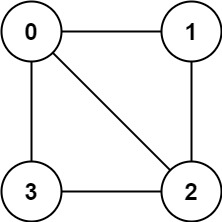
\includegraphics[width=.9\linewidth]{./img/bi2.jpg}
\caption{Example graph 1}
\end{figure}

\begin{verbatim}
Input: graph = [[1,2,3],[0,2],[0,1,3],[0,2]]
Output: false
\end{verbatim}

\begin{description}
\item[{Explanation}] There is no way to partition the nodes into two independent sets such that every edge connects a node in one and a node in the other.
\end{description}

\subsubsection{Example 2:}
\label{sec:org6e51b85}
\begin{figure}[htbp]
\centering
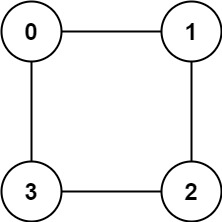
\includegraphics[width=.9\linewidth]{./img/bi1.jpg}
\caption{Example graph 2}
\end{figure}

\begin{verbatim}
Input: graph = [[1,3],[0,2],[1,3],[0,2]]
Output: true
\end{verbatim}
\textbf{Explanation:} We can partition the nodes into two sets: \{0, 2\} and \{1, 3\}.

\subsection{Constraints:}
\label{sec:org6e85f07}
\begin{itemize}
\item \texttt{graph.length == n}
\item \texttt{1 <= n <= 100}
\item \texttt{0 <= graph[u].length < n}
\item \texttt{0 <= graph[u][i] <= n - 1}
\item \texttt{graph[u]} does not contain \texttt{u}.
\item All the values of \texttt{graph[u]} are unique.
\item If \texttt{graph[u]} contains \texttt{v}, then \texttt{graph[v]} contains \texttt{u}.
\end{itemize}


\subsection{Analysis}
\label{sec:orgf968ab3}
The obvious approach is to use BFS or DFS to traverse the graph.

\subsection{Solutions}
\label{sec:orgffb60b3}
\subsubsection{Bipartite Graph solution using BFS}
\label{sec:org944f4a1}
\begin{verbatim}
#include <iostream>
#include <queue>
#include <vector>

using std::vector;
using std::queue;

bool bfs(int node, int color, vector<vector<int>>& graph, vector <int>& visited) {
    queue <int> q;
    q.push(node);
    visited[node] = color;
    while (!q.empty()) {
        int curr = q.front();
        q.pop();
        for (auto adjNode: graph[curr]) {
            if (visited[adjNode] == -1) {
                q.push(adjNode);
                visited[adjNode] = !visited[curr];
            } else if (visited[adjNode] == visited[curr]) {
                return false;
            }
        }
    }
    return true;
}
bool isBipartite(vector<vector<int>>& graph) {
    int n = graph.size(); // Get the node number
    vector <int> visited(n, -1); // Create visited vector for every node
    for (int i = 0; i < n; i++) {
        if (visited[i] == -1) {
            if (bfs(i, 0, graph, visited) == false)
                return false;
        }
    }
    return true;
}
\end{verbatim}

Similatrly, we can use DFS instead of BFS

\subsubsection{Bipartite Graph solution using DFS}
\label{sec:org89d9225}
\begin{verbatim}
#include <iostream>
#include <vector>

using std::vector;

bool dfs(int node, int color, vector<vector<int>>& graph, vector <int>& visited) {
    visited[node] = color;
    for (auto adjNode: graph[node]) {
        if (visited[adjNode] == -1) {
            if (dfs(adjNode, !color, graph, visited) == false)
                return false;
        } else if (visited[adjNode] == color) {
            return false;
        }
    }
    return true;
}

bool isBipartite(vector<vector<int>>& graph) {
    int n = graph.size();
    vector <int> visited(n, -1);
    for (int i = 0; i < n; i++) {
        if (visited[i] == -1) {
            if (dfs(i, 0, graph, visited) == false)
                return false;
        }
    }
    return true;
}
\end{verbatim}

But this is a primer on how we can utilize \texttt{Union-Find}.

\subsubsection{Bipartite Graph solution using Union-Find}
\label{sec:org3727cfe}

\begin{verbatim}
#include <iostream>
#include <vector>
#include <utility> // For std::pair

using std::vector;
using std::pair;


int find(vector<pair<int,int>> &parent, int k){
    if(parent[k].first == -1 || parent[k].first==k){
        parent[k].first = k;
        return k;
    }
    parent[k].first=find(parent,parent[k].first);
    return parent[k].first;
}

void unionFind(vector<pair<int,int>> &parent, int x, int y){
   int a = find(parent,x);
    int b = find(parent,y);
    if(a != b){
       if(parent[a].second < parent[b].second){
		   parent[a].first=b;
	   }else if(parent[a].second > parent[b].second){
			parent[b].first=a;
		}else{
			parent[b].first=a;
			parent[a].second += 1;
		}
    }
}
bool isBipartite(vector<vector<int>>& graph) {
    int n =graph.size();
    vector<pair<int,int>> parent(n,{-1,0});
    for(int i=0;i<n;i++){
        for(int j=0;j<graph[i].size();j++){
		 // node and neighbour shouldn't belong to same set in bipartite
            if(find(parent,i) == find(parent,graph[i][j])){
                return false;
            }
			// all node neighbours should belong to one set
            unionFind(parent,graph[i][j],graph[i][0]);
        }
    }
    return true;
}
\end{verbatim}

\section{Reverse Pairs}
\label{sec:org60b035a}
Given an integer array \texttt{nums}, return the number of \emph{reverse pairs} in the array.

A \emph{reverse pair} is a pair \texttt{(i, j)} where:
\begin{itemize}
\item \texttt{0 <= i < j < nums.length} and
\item \texttt{nums[i] > 2 * nums[j]}.
\end{itemize}

\subsection{Examples:}
\label{sec:orge49be1b}
\subsubsection{Example 1:}
\label{sec:orgc611f2b}
\begin{verbatim}
Input: nums = [1,3,2,3,1]
Output: 2
\end{verbatim}
\begin{description}
\item[{Explanation}] The reverse pairs are:
\begin{verbatim}
  (1, 4) --> nums[1] = 3, nums[4] = 1, 3 > 2 * 1
  (3, 4) --> nums[3] = 3, nums[4] = 1, 3 > 2 * 1
\end{verbatim}
\end{description}

\subsubsection{Example 2:}
\label{sec:org6b00e93}
\begin{verbatim}
Input: nums = [2,4,3,5,1]
Output: 3
\end{verbatim}
\begin{description}
\item[{Explanation}] The reverse pairs are:
\begin{verbatim}
  (1, 4) --> nums[1] = 4, nums[4] = 1, 4 > 2 * 1
  (2, 4) --> nums[2] = 3, nums[4] = 1, 3 > 2 * 1
  (3, 4) --> nums[3] = 5, nums[4] = 1, 5 > 2 * 1
\end{verbatim}
\end{description}

\subsection{Constraints:}
\label{sec:org07ea4d3}
\begin{itemize}
\item \(1 <= ~nums.length~ <= 5 * 10^4\)
\item \(-2^{31} <= ~nums[i]~ <= 2^{31} - 1\)
\end{itemize}

\subsection{Solution}
\label{sec:org6c5fd73}
\subsubsection{Using Divide and Conquer and Merge sort}
\label{sec:org439f7b9}
\begin{verbatim}
class Solution {
public:
    int inversions=0;
    int find_index_where_just_greater(int left,int right,vector<int>&arr,int target)
    {
        while(left<=right)
        {
            int mid=(left+right)/2;
            long long x=arr[mid];
            x*=2;
            if(x>=target)
            {
                right=mid-1;
            }
            else
            {
                left=mid+1;
            }
        }
        return (left-1);
    }
    void merge(vector<int>&arr,int l,int m,int r)
    {
        vector<int>Arr(r-l+1);
        int ptr1=l,ptr2=m+1,ptr3=0;
        while(ptr3<=(r-l))
        {
            if(ptr1==(m+1))
            {
                Arr[ptr3]=arr[ptr2];
                ptr2++;
                ptr3++;
                continue;
            }
            if(ptr2==(r+1))
            {
                int idx=find_index_where_just_greater(m+1,r,arr,arr[ptr1]);
                inversions+=idx-m;
                Arr[ptr3]=arr[ptr1];
                ptr1++;
                ptr3++;
                continue;
            }
            if(arr[ptr1]<=arr[ptr2])
            {
                int idx=find_index_where_just_greater(m+1,r,arr,arr[ptr1]);
                inversions+=idx-m;
                Arr[ptr3]=arr[ptr1];
                ptr1++;
                ptr3++;
            }
            else
            {
                Arr[ptr3]=arr[ptr2];
                ptr2++;
                ptr3++;
            }
        }
        for(int i=l;i<=r;i++)
        {
            arr[i]=Arr[i-l];
        }
        return;
    }
    void mergeSort(vector<int>&arr,int l,int r)
    {
        if(l==r)
        {
            return;
        }
        int mid=(l+r)/2;
        mergeSort(arr,l,mid);
        mergeSort(arr,mid+1,r);
        merge(arr,l,mid,r);
        return;
    }
    int reversePairs(vector<int>&nums)
    {
        mergeSort(nums,0,nums.size()-1);
        return inversions;
    }
};
\end{verbatim}

\subsubsection{Using segment tree}
\label{sec:org3d5df44}
\begin{verbatim}
int seg[1000006];
void update(int ind, int st, int en, int index) {
    if(st == en) {
        seg[ind]++;
        return;
    }
    int mid = (st + en) >> 1;
    if(index <= mid) {
        update(2 * ind + 1, st, mid, index);
    }
    else {
        update(2 * ind + 2, mid + 1, en, index);
    }
    seg[ind] = seg[2 * ind + 1] + seg[2 * ind + 2];
}
int query(int ind, int st, int en, int l, int r) {
    if(en < l || st > r || st > en) {
        return 0;
    }
    if(l <= st && en <= r) {
        return seg[ind];
    }
    int mid = (st + en) >> 1;
    return query(2 * ind + 1, st, mid, l, r) + query(2 * ind + 2, mid + 1, en, l, r);
}
int reversePairs(vector<int>& nums) {
    int n = nums.size();
    set<long long> st(nums.begin(), nums.end());
    int cnt = 0;
    unordered_map<int, int> mp;
    for(int i : st) {
        mp[i] = cnt++;
    }
    int ans = 0;
    for(int i = 0; i < n; i++) {
        long long rq = nums[i] * 2ll + 1;
        if(st.find(rq) != st.end()) {
            int l = mp[rq], r = n - 1;
            ans += query(0, 0, n - 1, l, r);
        }
        else {
            auto it = st.lower_bound(rq);
            if(it != st.end()) {
                int l = mp[*it], r = n - 1;
                ans += query(0, 0, n - 1, l, r);
            }
        }
        update(0, 0, n - 1, mp[nums[i]]);
    }
    return ans;
}
\end{verbatim}
\end{document}